\documentclass[10pt]{beamer}
\usetheme[
%%% option passed to the outer theme
%    progressstyle=fixedCircCnt,   % fixedCircCnt, movingCircCnt (moving is deault)
  ]{Feather}
%-------------------------------------------------------
% INCLUDE PACKAGES
%-------------------------------------------------------

\usepackage[utf8]{inputenc}
\usepackage[english]{babel}
\usepackage[T1]{fontenc}
\usepackage{helvet}


%-------------------------------------------------------
% Hack for hyperref warnings from the pdflatex compiler
%-------------------------------------------------------
\pdfstringdefDisableCommands{%
  \def\\{}%
}

%-------------------------------------------------------
% DEFFINING AND REDEFINING COMMANDS
%-------------------------------------------------------

% colored hyperlinks
\newcommand{\chref}[2]{
  \href{#1}{{\usebeamercolor[bg]{Feather}#2}}
}

%-------------------------------------------------------
% INFORMATION IN THE TITLE PAGE
%-------------------------------------------------------

\title[Religion, Meet Science] % [] is optional - is placed on the bottom of the sidebar on every slide
{ % is placed on the title page
      \textbf{Religion, Meet Science}
}

\subtitle{\textit{(Chapter 3)}}

\author{
	Brennan Fieck, Brionna Dumlao\\
    Nathan Fishel, Erin Hamand \\
    Kendyll Hawkins, Kris Lide \\
	Matthew McDonald, Zacary Parkhill
}

\date{\today}

%-------------------------------------------------------
% THE BODY OF THE PRESENTATION
%-------------------------------------------------------

\begin{document}

%-------------------------------------------------------
% THE TITLEPAGE
%-------------------------------------------------------

{\1% % this is the name of the PDF file for the background
\begin{frame}[plain,noframenumbering] % the plain option removes the header from the title page, noframenumbering removes the numbering of this frame only
  \titlepage % call the title page information from above
\end{frame}}


\begin{frame}{Content}{}
\tableofcontents
\end{frame}

%-------------------------------------------------------
\section{In the Beginning}
\subsection{The United States}
%-------------------------------------------------------
\begin{frame}{In the Beginning}{The United States}
%-------------------------------------------------------
	\begin{itemize}
		\item<1 -> Settled by Christians - the Puritans.
		\item<2 -> Founded on science - logic and reason.
			\begin{itemize}
				\item<3 -> Logic and reason helped ensure religious freedom
				\item<3 -> This is why religious mentality was not incorporated into the Declaration of Independence
			\end{itemize}
	\end{itemize}
\end{frame}

%-------------------------------------------------------
\subsection{God's Natural Law is Reason}
%-------------------------------------------------------
\begin{frame}{In the Beginning}{God's Natural Law is Reason}
%-------------------------------------------------------
	\begin{columns}[T]
		\column{0.6\textwidth}
			From approx. 700 C.E. to 900 C.E.\\
			\begin{itemize}
				\item Mu'tazilites mode of study
					\begin{itemize}
						\item Discern God's will by studying nature
						\item God speaks through nature
					\end{itemize}
			\end{itemize}
		\column{0.4\textwidth}
			\begin{figure}
				\centering
				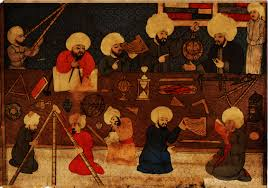
\includegraphics[width=\textwidth]{images/mutazilite_science}
				\caption{Mu'tazilite Science}
			\end{figure}
	\end{columns}
\end{frame}

%-------------------------------------------------------
\begin{frame}{In the Beginning}{God's Natural Law is Reason}
%-------------------------------------------------------
	\begin{columns}[T]
		\column{0.6\textwidth}
			1517 C.E.
			\begin{itemize}
				\item Martin Luther nails his 95 theses to the door of a Catholic church to protest the Church's practices
					\begin{itemize}
						\item Protestants argued that knowledge comes from observing God's Word, not the Pope's word
					\end{itemize}
			\end{itemize}
		\column{0.4\textwidth}
			\begin{figure}
				\centering
				
\includegraphics[width=\textwidth]{images/martin_luther}
				\caption{Martin Luther}
			\end{figure}
	\end{columns}
\end{frame}

%-------------------------------------------------------
\begin{frame}{In the Beginning}{God's Natural Law is Reason}
%-------------------------------------------------------
	\begin{columns}[T]
		\column{0.6\textwidth}
			1518 C.E.
			\begin{itemize}
				\item Protestant polemicist St. Germain supports "do it yourself" Bible study
					\begin{itemize}
						\item Protestants argued that knowledge comes from observing God's Word, not the Pope's word
						\item Use one's own experience of the Bible to find truth\\
							This approach is in the same "anti-authoritarian" vein as the modern scientific approach (make observations, then come to conclusions)
					\end{itemize}
			\end{itemize}
		\column{0.4\textwidth}
			\begin{figure}
				\centering
				
\includegraphics[width=\textwidth]{images/martin_luther}
				\caption{Martin Luther}
			\end{figure}
	\end{columns}
\end{frame}

%-------------------------------------------------------
\begin{frame}{In the Beginning}{God's Natural Law is Reason}
%-------------------------------------------------------
	\begin{columns}[T]
		\column{0.6\textwidth}
			Early 1600's
			\begin{itemize}
				\item Puritan sympathizer Edward Coke argues that scientific laws could be studied by everyone, and could not be overruled by the crown.
			\end{itemize}
		\column{0.4\textwidth}
			\begin{figure}
				\centering
				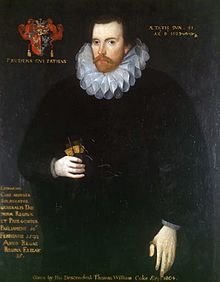
\includegraphics[width=\textwidth]{images/edward_coke}
				\caption{Edward Coke}
			\end{figure}
	\end{columns}
\end{frame}

%-------------------------------------------------------
\begin{frame}{In the Beginning}{God's Natural Law is Reason}
%-------------------------------------------------------
	\begin{columns}[T]
		\column{0.6\textwidth}
			Late 1500's to mid 1600's
			\begin{itemize}
				\item Puritans supported a logical, antiauthoritarian approach to theology:
					\begin{itemize}
						\item Making your own observations from the Bible and not relying on the Pope
						\item Use observations to draw broader theological conclusions
						\item Puritans study Mu'tazilite science books
					\end{itemize}
			\end{itemize}
		\column{0.4\textwidth}
			\begin{figure}
				\centering
				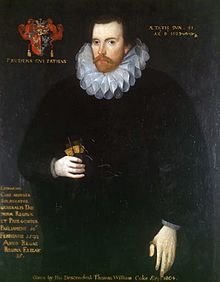
\includegraphics[width=\textwidth]{images/edward_coke.png}
				\caption{Edward Coke}
			\end{figure}
	\end{columns}
\end{frame}



% Timeline of Events:

% ~A.D. 700-900: Mu’tazilites mode of study: Discern God’s will by studying nature
% God speaks through nature
% 1517: Beginning of the Protestant Reformation 
% Martin Luther nails his 95 Theses, in protest of the Catholic Church’s practices
% Protestants argued that knowledge comes from observing God’s Word, not the Pope’s word
% 1518: Protestant polemicist St. Germain supports “do it yourself” Bible study
%           - Use one own’s experience of the Bible to find truth
%           - This approach used was of the same “antiauthoritarian” nature of the emerging (now modern) scientific approach (make observations, then come to conclusion)

% Early 1600s: Puritan sympathizer Edward Coke argues that scientific laws could be studied by everyone, and could not be overruled by the crown.

% Late 1500s to mid-1600s:  Puritans supported a logical, antiauthoritarian approach to theology:
% Making your own observations from the Bible and not relying on the Pope
% Use observations to draw broader theological conclusions
% Puritans study Mu’tazilite science books


%-------------------------------------------------------
\section{How Do We Know Things?}
%-------------------------------------------------------
%\subsection{License}
\begin{frame}{How Do We \textit{Know} Things?}{(auth. Brennan Fieck)} % I'm still torn on the attribution line, but it seems like a good idea for the time being.
%-------------------------------------------------------

  \begin{itemize}
    \item The Feather image is not covered by copyright rules. I have used the image from \chref{http://www.vectors-free.com/}{http://www.vectors-free.com/}. You are allowed to use the Feather image for any purposes.
    \item The rest of the theme is provided under the GNU General Public License v. 3 (GPLv3) \chref{http://www.gnu.org/licenses/}{http://www.gnu.org/licenses/}. This means that you can redistribute it and/or modify it under the same license. 
  \end{itemize}
\end{frame}

%-------------------------------------------------------
\section{Installation}
%-------------------------------------------------------
\subsection{Source files}
\begin{frame}{Installation}{Source files}
%-------------------------------------------------------

\begin{block}{}
The theme contains 4 source files:
  \begin{itemize}
    \item {\tt beamercolorthemeFeather.sty}
    \item {\tt beamerouterthemeFeather.sty}
    \item {\tt beamerinnerthemeFeather.sty}
    \item {\tt beamerthemeFeather.sty}
  \end{itemize}
\end{block}
\end{frame}

%-------------------------------------------------------
\subsection{Local and Global installation}
\begin{frame}{Installation}{Local and Global installation}
%-------------------------------------------------------
  The theme can be installed for \textbf{local} or \textbf{global} use.
  \pause
  \begin{block}{Local Installation}
  \begin{itemize}    
    \item Local installation is the simplest way of installing the theme. 
    \item You need to placing the 4 source files in the same folder as your presentation. When you download the theme, the 4 theme files are located in the {\tt local} folder.
  \end{itemize}
  \end{block}

  \begin{block}{Global Installation}
  \begin{itemize}
     \item If you wish to make the theme globally available, you must put the files in your local latex directory tree. The location of the root of the local directory tree depends on your operating system and the latex distribution. 
     \item Detailed steps on how to proceed installation under various operating systems can be found at Beamer documentation.
  \end{itemize}
  \end{block}
\end{frame}
     

%-------------------------------------------------------
\subsection{Required Packages}
\begin{frame}{Installation}{Required Packages}
%-------------------------------------------------------

  For using the Feather Theme you will need the Bemaer class installed and the following 2 packages
  \begin{itemize}
    \item TikZ\footnote{TikZ is a package for creating beautiful graphics. Have a look at these \chref{http://www.texample.net/tikz/examples/}{online examples} or the \chref{http://tug.ctan.org/tex-archive/graphics/pgf/base/doc/generic/pgf/pgfmanual.pdf}{pgf user manual}.}
    \item calc
  \end{itemize}
  Due to the fact that the packages are very common they should be included in your latex distribution in the first place.
\end{frame}

%-------------------------------------------------------
\section{User Interface}
\subsection{Loading the Theme and Theme Options}
\begin{frame}{User Interface}{Loading the Theme and Theme Options}
%-------------------------------------------------------

  \begin{block}{The Presentation Theme}
    The Feather Theme can be loaded in a familiar way. In the reamble of your {\tt tex} file you must type\\ \vspace{5pt} 
    {\tt \textbackslash usetheme[<options>]\{Feather\}}\\ \vspace{5pt} 
    The presentation theme loads the inner, outer and color Feather theme files and passes the {\tt <options>} on to these files.
  \end{block}
  \begin{block}{The Inner and Outher Themes}
    If you wish you can load only the inner, or the outher theme directly by\\ \vspace{5pt} 
    {\tt \textbackslash useinnertheme\{Feather\}} (and it has no options)\\ \vspace{5pt} 
    {\tt \textbackslash useoutertheme[<options>]\{Feather\}} (it has one option)\\
    \hspace{20pt}{\tt progressstyle=\{fixedCircCnt or movingCircCnt\}} \\
    \begin{itemize}
    \item which set how the progress is illustrated;
    \item the value {\tt movingCircCnt} is the default.
    \end{itemize}
  \end{block}
\end{frame}

\begin{frame}{User Interface}{Loading the Theme and Theme Options}

  \begin{block}{The Color Theme}
    Also you can load only the color theme by writing in the preamble of the {\tt tex} file 
    
    \vspace{5pt} 
    
    \begin{itemize}
    \item {\tt \textbackslash usecolortheme\{Feather\}}
    \end{itemize}
    
    \vspace{5pt}
    
    ...or to change the colors of the various elements in the theme
    
    \vspace{5pt} 
    \begin{itemize}
    \item Change the bar colors: \\    
    {\tt \textbackslash setbeamercolor \{Feather\}\{fg=<color>, bg=<color>\}}
    
    \vspace{2pt} 
    
    \item Change the color of the structural elements: \\    
    {\tt \textbackslash setbeamercolor\{structure\}\{fg=<color>\}}
    
    \vspace{2pt} 
    
    \item Change the frame title text color:\\
    {\tt \textbackslash setbeamercolor\{frametitle\}\{fg=<color>\}}
    
    \vspace{2pt} 
    
    \item Change the normal text color background:    
    {\tt \textbackslash setbeamercolor\{normal text\}\{fg=<color>, bg=<color>\}}
    \end{itemize}
  \end{block}
\end{frame}


%-------------------------------------------------------
\subsection{Feather image}
\begin{frame}{User Interface}{The Feather Background Image}
%-------------------------------------------------------

\begin{block}{The Feather Background Image}
    \begin{itemize}
    \item In Feather theme, the title page frame and the last frame have the Feather image as the background image. 
    \item The Feather background image can be produced to any frame by wrating on the begining at the choosen frame the following
    \end{itemize} 
    
    \vspace{5pt} 
    
  {\tt \{\textbackslash 1bg\\
    \textbackslash begin\{frame\}[<options>]\{Frame Title\}\{Frame Subtitle\}\\
    \ldots\\
    \textbackslash end\{frame\}\}}
\end{block}
\end{frame}


{\1
\begin{frame}[plain,noframenumbering]
  \finalpage{Thank you for using Feather Beamer Theme!}
\end{frame}}

\end{document}